% === Yêu cầu package trong preamble ===
% \usepackage{pgfplots}
% \usepackage{tikz}
% \pgfplotsset{compat=1.18}

\begin{figure}[t]
\centering
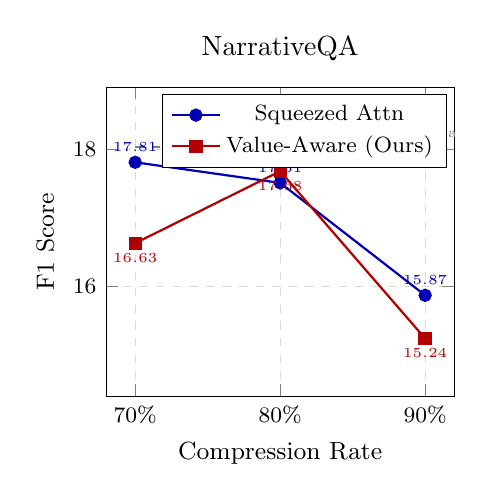
\begin{tikzpicture}
\begin{axis}[
    width=6cm,
    height=5.5cm,
    title={NarrativeQA},
    ylabel={F1 Score},
    xlabel={Compression Rate},
    enlarge x limits=0.1,
    ylabel style={font=\small},
    xlabel style={font=\small},
    tick label style={font=\footnotesize},
    legend style={font=\footnotesize, at={(0.98,0.98)}, anchor=north east},
    grid=major,
    grid style={dashed, gray!30},
    symbolic x coords={70\%, 80\%, 90\%},
    xtick=data,
    ymin=14.4,
    ymax=18.9,
]
\addplot[gray, thick, dashed, forget plot, domain=0:2, samples=2] coordinates {
    (70\%, 18.03)
    (90\%, 18.03)
};
\node[gray, font=\tiny, anchor=south west] at (axis cs:90\%, 18.03) {Baseline};
\addplot[color=blue!70!black, mark=*, thick, nodes near coords, every node near coord/.append style={font=\tiny, anchor=south}] coordinates {
    (70\%, 17.81)
    (80\%, 17.51)
    (90\%, 15.87)
};
\addplot[color=red!70!black, mark=square*, thick, nodes near coords, every node near coord/.append style={font=\tiny, anchor=north}] coordinates {
    (70\%, 16.63)
    (80\%, 17.68)
    (90\%, 15.24)
};
\legend{Squeezed Attn, Value-Aware (Ours)}
\end{axis}
\end{tikzpicture}
\caption{Performance on NarrativeQA.}
\label{fig:results_narrativeqa}
\end{figure}